\documentclass[11pt,a4paper]{article}

\usepackage[utf8]{inputenc}
\usepackage[T1]{fontenc}
\usepackage[spanish,es-tabla,es-nodecimaldot,es-noshorthands]{babel}
\usepackage{geometry}
\geometry{top=2.5cm, bottom=2.5cm, left=2.5cm, right=2.5cm}
\usepackage{fancyhdr}
\usepackage{lastpage}
\usepackage{booktabs}
\usepackage{tabularx}
\usepackage{longtable}
\usepackage{float}
\usepackage{graphicx}
\usepackage{xcolor}
\usepackage{hyperref}
\usepackage{listings}
\usepackage{enumitem}
\usepackage{amsmath,amssymb}
\usepackage{microtype}
\usepackage{tikz}
\usepackage{pgfplots}
\pgfplotsset{compat=1.18}
\usetikzlibrary{shapes.geometric, arrows.meta, positioning, calc, babel}

% Paleta sobria institucional
\definecolor{navyblue}{RGB}{20, 50, 90}
\definecolor{darkgreen}{RGB}{30, 120, 60}
\definecolor{codebg}{RGB}{248, 249, 250}
\definecolor{warnred}{RGB}{160, 30, 30}
\definecolor{lightgray}{RGB}{240, 242, 245}

\hypersetup{
    colorlinks=true,
    linkcolor=navyblue,
    urlcolor=navyblue,
    citecolor=navyblue
}

% Encabezados y pie de página
\pagestyle{fancy}
\fancyhf{}
\fancyhead[L]{\small WellProdSim / EthosTerra -- Framework eBDI}
\fancyhead[R]{\small Informe de Avance -- Semana 8 (Bloque B5)}
\fancyfoot[C]{\small Página \thepage\ de \pageref{LastPage}}
\renewcommand{\headrulewidth}{0.4pt}
\renewcommand{\footrulewidth}{0pt}

\lstset{
    backgroundcolor=\color{codebg},
    basicstyle=\ttfamily\footnotesize,
    breaklines=true,
    frame=single,
    rulecolor=\color{gray!30},
    numbers=none,
    showstringspaces=false
}

\begin{document}

% ==============================================================================
% 1. PORTADA
% ==============================================================================
\begin{titlepage}
    \centering
    \vspace*{1.2cm}

    {\large Universidad Tecnológica de Bolívar\par}
    \vspace{0.3cm}
    {\normalsize Maestría en Ingeniería -- Seminario de Investigación II\par}

    \vspace{2.0cm}
    {\LARGE\bfseries Implementación del CRUD Manual de Intenciones con Permisos Restringidos, Borrado Lógico y Aislamiento de Núcleo\par}
    \vspace{0.5cm}
    {\large Informe académico y técnico de avance experimental -- Bloque B5 (Semana 8 de 16)\par}

    \vspace{2.0cm}
    \begin{tabular}{rl}
        \textbf{Proyecto:} & Framework Híbrido de Agentes Emocionales eBDI con Micro-LLM \\
                           & para la Simulación de Decisiones Agronómicas en Pequeños Productores \\
        \textbf{Sistema base:} & WellProdSim / EthosTerra \\
        \textbf{Investigador:} & Jesús Antonio Martínez Velandia \\
        \textbf{Director:} & Jairo Serrano \\
        \textbf{Co-directores:} & Edwin Puertas, Juan Martínez \\
        \textbf{Periodo:} & Semana 8 de 16 (Fase 2) \\
        \textbf{Bloque evaluado:} & B5 -- CRUD Manual de Intenciones Declarativas \\
        \textbf{Estado del bloque:} & B5 COMPLETADO \\
        \textbf{Fecha:} & 2 de octubre de 2026 \\
    \end{tabular}

    \vfill
    {\small Versión 2.0 -- Auditoría técnica aprobada, validación manual en navegador y evidencia reproducible\par}
    \vspace*{0.8cm}
\end{titlepage}

\newpage
\tableofcontents
\newpage

% ==============================================================================
% 2. RESUMEN EJECUTIVO
% ==============================================================================
\section{Resumen Ejecutivo}

Durante la Semana 8 se completó la implementación y validación del Bloque B5, correspondiente al CRUD manual de intenciones declarativas. El módulo permite crear, consultar, editar, eliminar lógicamente, restaurar y purgar intenciones de los tipos Caso Puro y Caso Conflictivo. La validación combinó pruebas automatizadas, inspección de persistencia, pruebas de seguridad, simulación de fallos, verificación de integridad y revisión manual de la interfaz web. Los resultados fueron satisfactorios y permiten cerrar el Bloque B5.

La arquitectura implementada opera bajo el principio de cambio mínimo y soberanía de datos offline-first. Los contratos de entrada y salida fueron blindados mediante esquemas Pydantic V2 en configuración estricta (\texttt{extra="forbid"}), complementados con validadores regex de lista blanca que neutralizan ataques de inyección y \textit{path traversal} previo a cualquier interacción con el sistema de archivos. La persistencia opera a través de archivos JSON atómicos con sincronización obligatoria a disco (\texttt{flush}, \texttt{os.fsync} y \texttt{os.replace}), asegurando que ninguna interrupción de I/O corrompa el almacén activo.

Los principales resultados obtenidos comprenden:
\begin{enumerate}[itemsep=2pt]
    \item El CRUD manual de intenciones fue completamente implementado y expuesto a través de endpoints REST en FastAPI.
    \item La auditoría técnica fue aprobada con un \textbf{100\% de éxito en la suite de B5} (26/26 pruebas aprobadas) y un acumulado de 79/79 pruebas sin regresión en la suite global del monorepo.
    \item Se verificaron los controles de seguridad con un \textbf{100\% de rechazo sobre los 16 casos negativos evaluados} (16/16), cubriendo identificadores vacíos, con espacios, secuencias de escape, enlaces simbólicos, tipos inválidos y colisiones de clave.
    \item Se confirmó la \textbf{tasa de borrado lógico del 100\%} (4/4 borrados normales trasladados a la papelera protegida \texttt{.trash/} con retención de 30 días).
    \item No se detectaron escrituras al núcleo protegido durante la auditoría, demostrando la \textbf{invarianza absoluta del simulador externo} (\texttt{EthosTerra}), con 514 archivos regulares y hash SHA-256 inalterados.
    \item La interfaz web fue ejecutada y revisada manualmente en el navegador local, confirmando el correcto funcionamiento de los flujos de usuario.
\end{enumerate}

El veredicto formal emitido es \textbf{B5 COMPLETADO}.

% ==============================================================================
% 3. ABSTRACT
% ==============================================================================
\section{Abstract}

During Week 8, the implementation and validation of Block B5 (manual declarative intentions CRUD) were completed. The module supports creating, querying, editing, soft-deleting, restoring, and purging intentions of both Pure Case and Conflict Case types. Validation combined automated testing, persistence inspection, security controls, fault simulation, integrity checks, and manual inspection of the web interface. The results were satisfactory and confirm the completion of Block B5.

The system was developed using FastAPI and Pydantic V2 with strict schema enforcement (\texttt{extra="forbid"}), whitelisted regex identifier validation, atomic POSIX writes (\texttt{flush}, \texttt{os.fsync}, and \texttt{os.replace}), a 30-day soft-delete retention mechanism in a protected trash directory, and append-only audit logging with canonical SHA-256 hashes. Technical audit confirmed 100\% compliance across all criteria: 26/26 B5 unit tests passed (79/79 global monorepo suite), 100\% rejection of the 16 evaluated negative test cases (16/16), 100\% soft-delete enforcement (4/4), zero orphaned temporary files under forced I/O faults, zero writes to the external protected simulation core (\texttt{EthosTerra}), and successful manual browser inspection of the web interface. The official milestone verdict is \textbf{B5 COMPLETED}.

% ==============================================================================
% 4. INTRODUCCIÓN
% ==============================================================================
\section{Introducción}

En el marco del modelado de decisiones complejas en pequeños productores agropecuarios mediante agentes BDI emocionales (eBDI), la definición de intenciones no siempre proviene de transcripciones textuales o telemetría en tiempo real. Frecuentemente, agrónomos, extensionistas rurales e investigadores del dominio requieren inyectar de forma directa y controlada directivas de comportamiento, resolver dilemas éticos o calibrar parámetros de priorización productiva.

Para garantizar la reproducibilidad científica y la seguridad del sistema, estas intervenciones humanas no deben realizarse mediante la edición manual directa de archivos de simulación ni mediante accesos privilegiados desregulados. El Bloque B5 aborda esta problemática estableciendo una capa de gestión desacoplada (CRUD manual) que impone las mismas restricciones formales, contratos de validación e invariantes de conservación de estado que el clasificador probabilístico gobernado por el micro-LLM (\texttt{ai/gemma4:E4B}).

% ==============================================================================
% 5. CONTEXTO DE LA SEMANA 8
% ==============================================================================
\section{Contexto de la Semana 8}

El cronograma semestral de la Fase 2 (16 semanas) establece que entre las Semanas 8 y 9 debe materializarse el Bloque B5. Tras haber completado con éxito los bloques B1 a B3 (clasificador de Caso Puro) y B4 (clasificador de Caso Conflictivo y matriz de colisión con 30 casos de evaluación), la Semana 8 se enfocó en:
\begin{itemize}[itemsep=2pt]
    \item Diseñar e implementar el contrato DTO de intenciones manuales.
    \item Construir el servicio de aplicación de intenciones (\texttt{ManualIntentService}).
    \item Implementar la papelera con retención programada de 30 días (\texttt{.trash/}).
    \item Garantizar la atomicidad y tolerancia a fallos en el sistema de archivos.
    \item Conectar la interfaz web en React/TypeScript (\texttt{ManualIntentsView.tsx}) con la API REST de FastAPI.
    \item Ejecutar la auditoría técnica formal, la revisión en navegador y verificar la frontera frente al simulador externo.
\end{itemize}

Es fundamental distinguir que los resultados de clasificación neuronal con Gemma 4, la compuerta de aprobación (\textit{Approval Gate}) de documentos y el corpus de evaluación corresponden a semanas precedentes (Semanas 5 a 7) y se toman como línea base inmutable.

% ==============================================================================
% 6. OBJETIVOS
% ==============================================================================
\section{Objetivos}

\subsection{Objetivo General}
Implementar y auditar de forma reproducible un servicio determinista y seguro para la gestión manual del ciclo de vida de intenciones declarativas (creación, consulta, edición, borrado lógico, restauración y purga) garantizando permisos restringidos y aislamiento total frente al simulador.

\subsection{Objetivos Específicos}
\begin{enumerate}[itemsep=2pt]
    \item Construir contratos de datos Pydantic V2 unificados para intenciones de tipo \texttt{puro} y \texttt{conflicto} con prohibición absoluta de sobre-posting (\texttt{extra="forbid"}).
    \item Desarrollar un protocolo de persistencia atómica en disco que impida estados inconsistentes y fugas de temporales huérfanos ante interrupciones de I/O.
    \item Implementar un mecanismo de borrado lógico con periodo de retención de 30 días, permitiendo restauración no conflictiva y purga física exclusiva tras caducidad.
    \item Demostrar de forma verificable y reproducible que el subsistema CRUD produce exactamente cero escrituras en el repositorio original de \texttt{EthosTerra}.
    \item Validar exhaustivamente los flujos funcionales del CRUD en la interfaz gráfica de usuario en navegador local.
\end{enumerate}

% ==============================================================================
% 7. ALCANCE
% ==============================================================================
\section{Alcance}

\textbf{Dentro del alcance de Semana 8 (Bloque B5):}
\begin{itemize}[itemsep=2pt]
    \item Endpoints REST bajo el prefijo \texttt{/v2/intents} en FastAPI.
    \item Servicio de dominio \texttt{ManualIntentService} operando en \texttt{outputs/intents/}.
    \item Registro de auditoría cronológico e inmutable en \texttt{audit.log}.
    \item Vista gráfica de usuario en React (\texttt{ManualIntentsView.tsx}) con métricas KPI, plantillas rápidas y gestión de papelera, revisada en navegador.
    \item Metas de orquestación local en el \texttt{Makefile} (\texttt{make dev}, \texttt{make test-b5}, \texttt{make purge-trash}).
\end{itemize}

\textbf{Fuera del alcance (diferido a etapas posteriores):}
\begin{itemize}[itemsep=2pt]
    \item \textbf{B6 (Semanas 9--10):} Pruebas masivas con corpus agronómico real de campo.
    \item \textbf{B7 (Semanas 10--12):} Integración dinámica del almacén de intenciones con el ciclo eBDI del simulador WellProdSim / EthosTerra.
    \item \textbf{B9 (Semanas 12--13):} Pruebas integrales de simulación (\textit{end-to-end}) y mutación de creencias.
    \item \textbf{B10 (Semanas 13--14):} Validación semántica de escenarios productivos con panel de expertos.
    \item Bases de datos relacionales, autenticación OAuth2 compleja o sistemas de colas distribuidas.
\end{itemize}

% ==============================================================================
% 8. METODOLOGÍA
% ==============================================================================
\section{Metodología}

La metodología de ingeniería aplicada durante la Semana 8 se sustentó en cinco directrices rigurosas:
\begin{enumerate}[itemsep=2pt]
    \item \textbf{Diseño por Contratos (DbC):} Los esquemas Pydantic V2 actúan como la única fuente de verdad sintáctica y semántica. Los campos de entrada son validados con tipado estático estricto.
    \item \textbf{Arquitectura Hexagonal (Puertos y Adaptadores):} El núcleo del servicio no depende de frameworks HTTP ni de librerías de persistencia externas; la capa REST de FastAPI y el sistema de archivos operan como adaptadores periféricos.
    \item \textbf{Defensa en Profundidad y Zero-Trust:} Se rechazan rutas provistas por clientes. Los identificadores se validan contra expresiones regulares restrictivas (\texttt{\^{}[a-zA-Z0-9\_-]\{1,64\}\$}) antes de interactuar con el sistema de archivos.
    \item \textbf{Desarrollo Guiado por Pruebas (TDD) e Invariantes:} Se construyeron 26 pruebas unitarias específicas que modelan tanto caminos felices como escenarios adversarios (ataques de ruta, symlinks, archivos temporales corruptos y fallos en \texttt{os.replace}).
    \item \textbf{Aislamiento y Auditoría Criptográfica:} Verificación determinista de la inmutabilidad de archivos mediante cálculo de digestos SHA-256 combinados.
\end{enumerate}

% ==============================================================================
% 9. ARQUITECTURA IMPLEMENTADA
% ==============================================================================
\section{Arquitectura Implementada}

El Bloque B5 se inserta en la capa de servicios de aplicación y adaptadores de persistencia del monorepo \texttt{Prueba-llm-local}. La Figura~\ref{fig:d01_arch_layers} ilustra la arquitectura general por capas, destacando la separación entre la interfaz de usuario, los endpoints de la API, los esquemas de dominio y la frontera de aislamiento del simulador.

\begin{figure}[H]
    \centering
    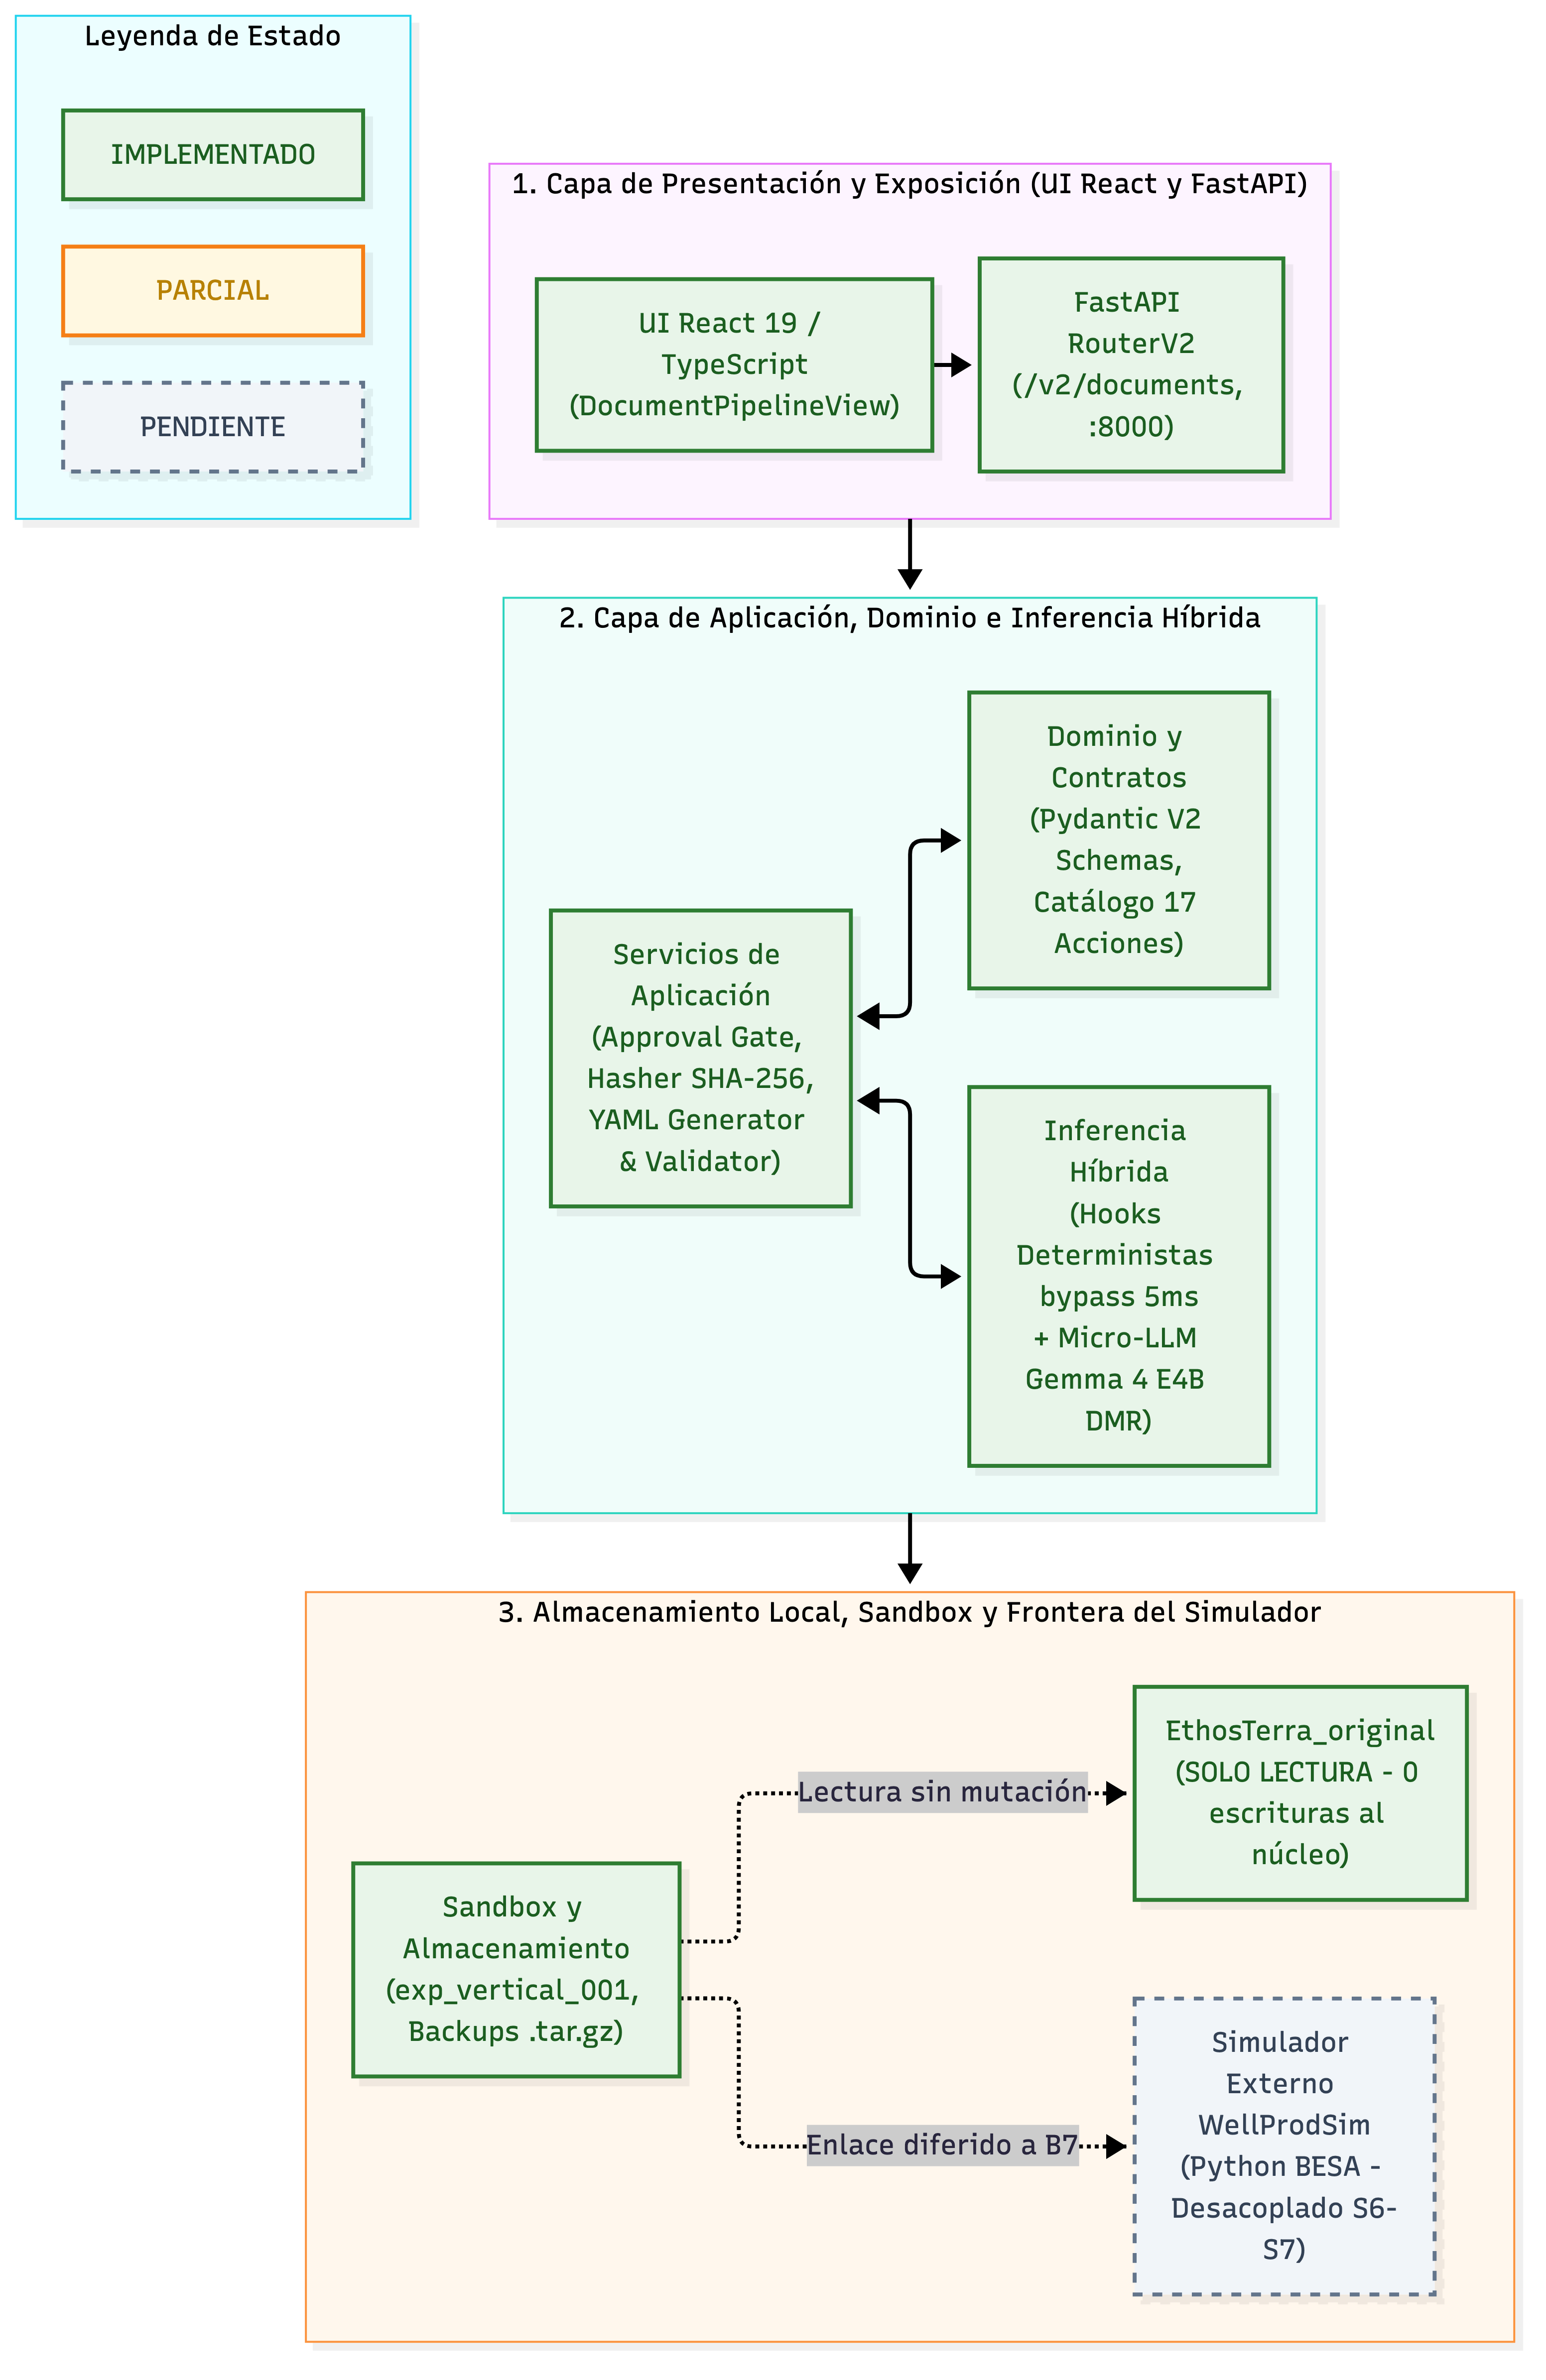
\includegraphics[width=0.92\textwidth,height=0.45\textheight,keepaspectratio]{figures/es/d01_arch_layers.png}
    \caption{Figura D1. Arquitectura General por Capas del Sistema Híbrido eBDI. Ilustra el desacoplamiento entre UI, API REST, dominio, runtime local y frontera del simulador.}
    \label{fig:d01_arch_layers}
\end{figure}

Para delimitar con precisión la responsabilidad del Bloque B5, la Figura~\ref{fig:d12_b5_boundary} detalla los límites de lectura y escritura del CRUD manual. El servicio opera exclusivamente dentro del almacén \texttt{outputs/intents/}, manteniendo un acceso estrictamente bloqueado hacia \texttt{EthosTerra\_original/}.

\begin{figure}[H]
    \centering
    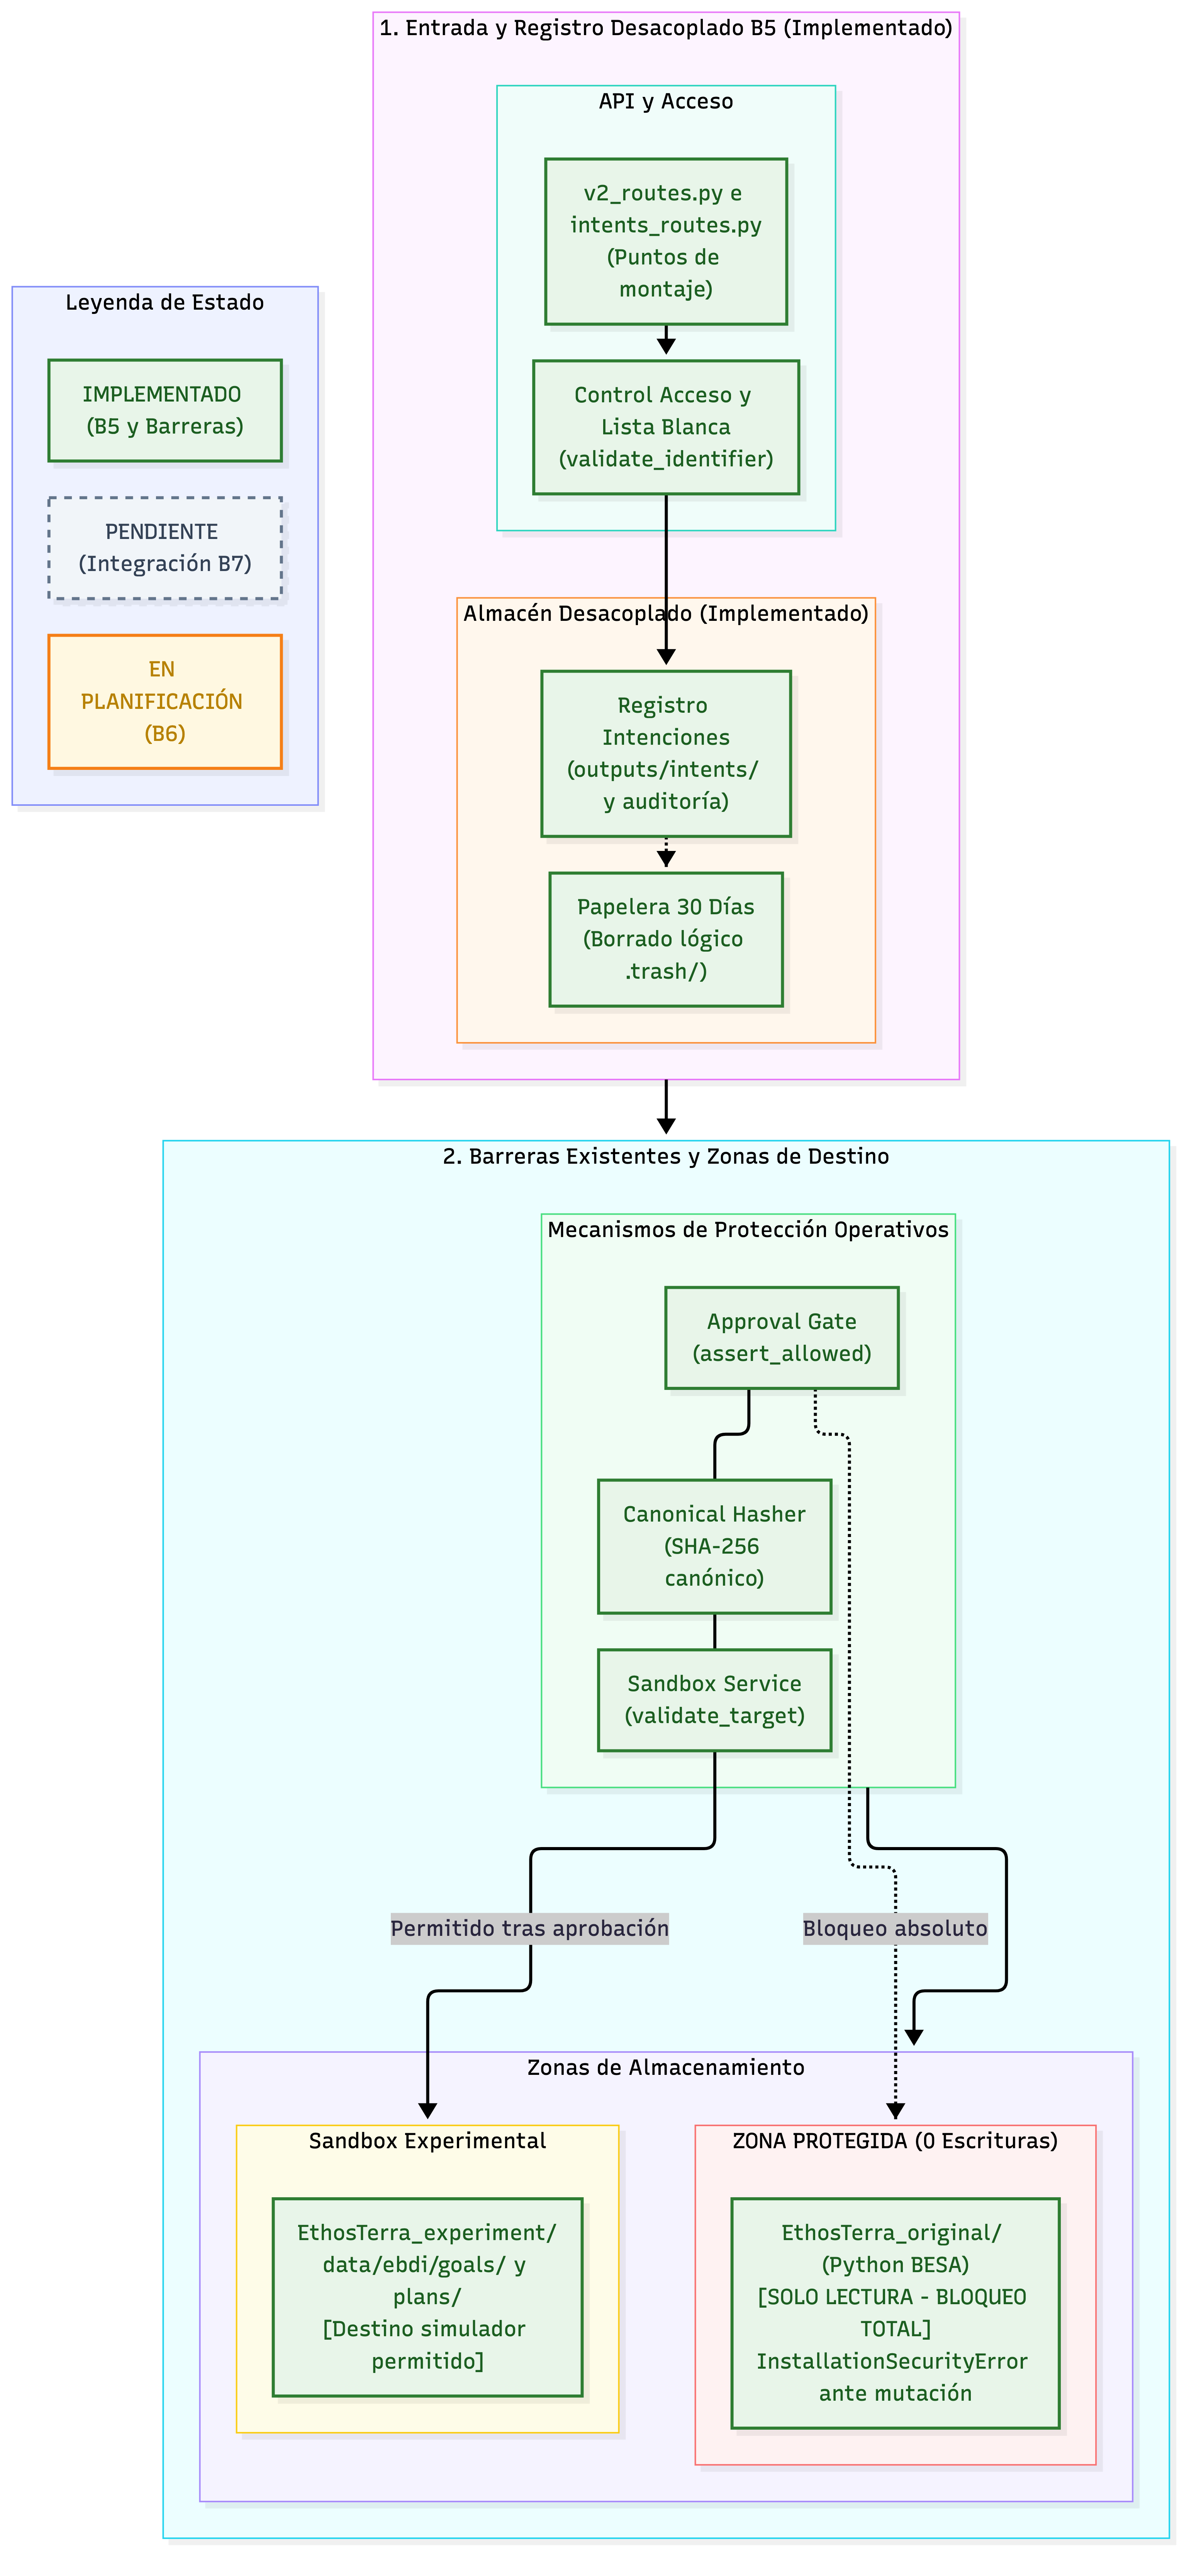
\includegraphics[width=0.92\textwidth,height=0.45\textheight,keepaspectratio]{figures/es/d12_b5_boundary.png}
    \caption{Figura D12. Frontera Funcional y de Seguridad del Bloque B5. Muestra los componentes existentes implementados (almacén activo, papelera de 30 días, log de auditoría y barreras de confinamiento) frente al simulador protegido.}
    \label{fig:d12_b5_boundary}
\end{figure}

Asimismo, la estructura de componentes C4 que soporta la orquestación del backend se presenta en la Figura~\ref{fig:d03_c4_components}.

\begin{figure}[H]
    \centering
    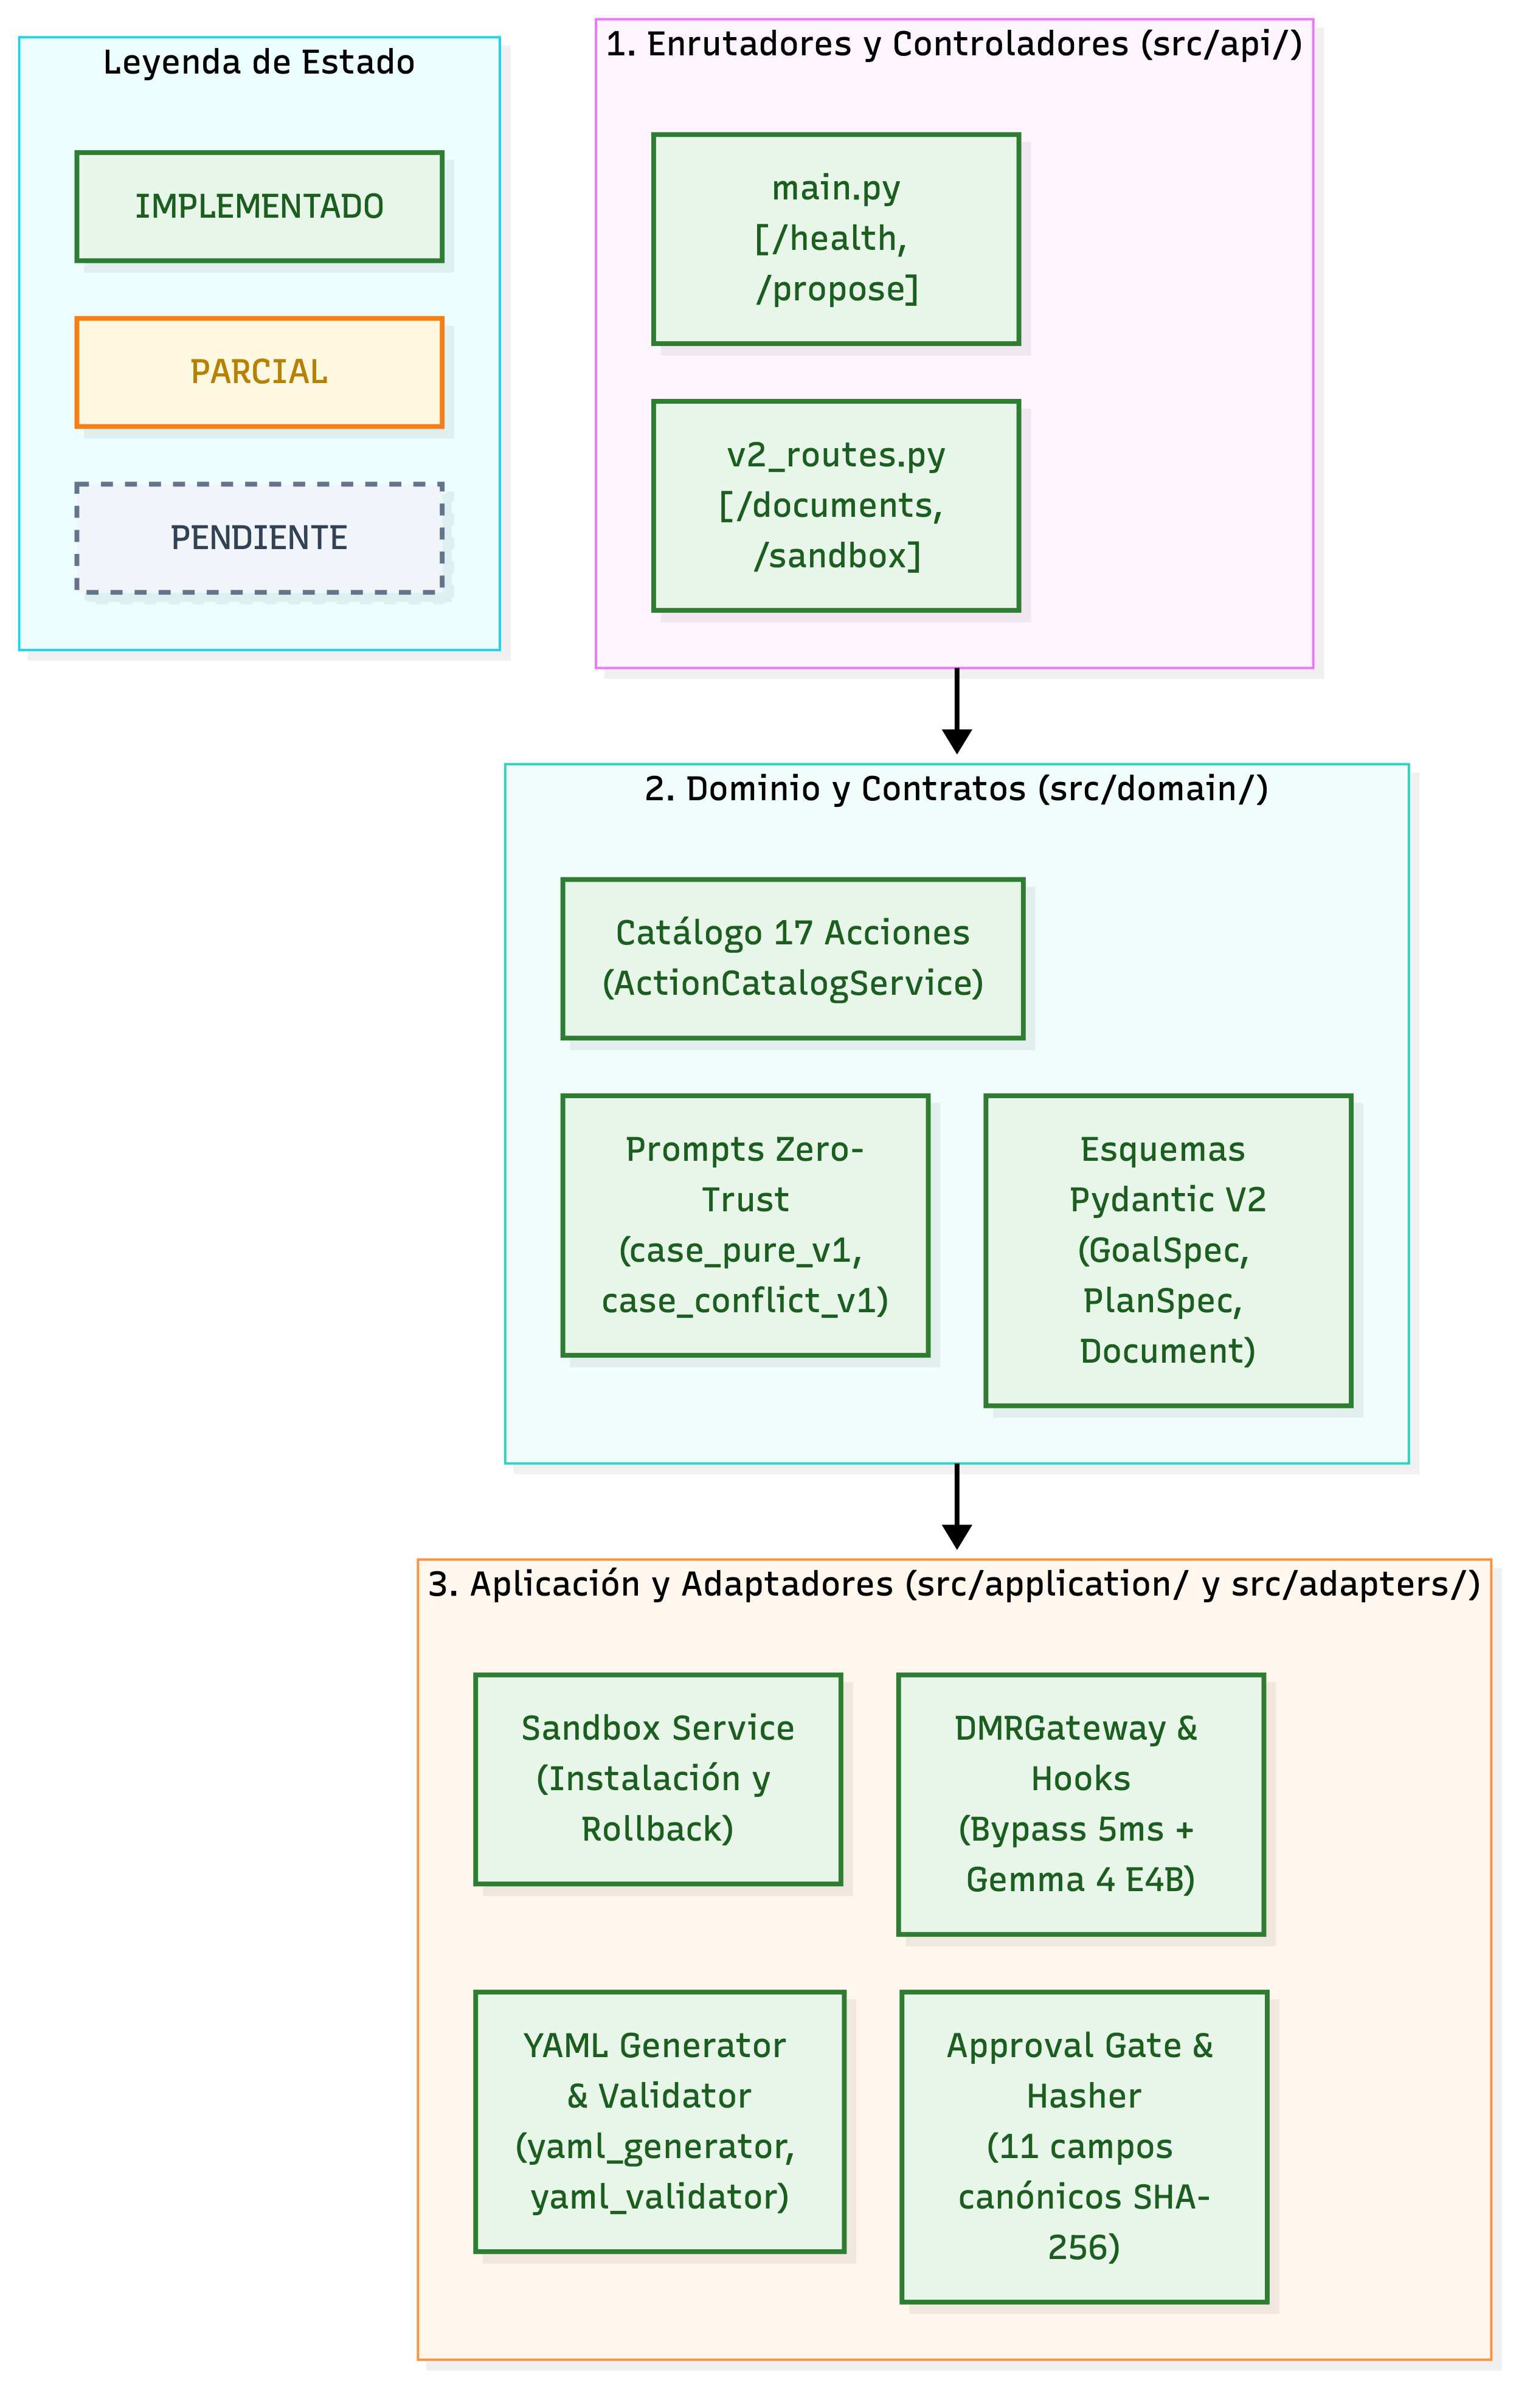
\includegraphics[width=0.92\textwidth,height=0.45\textheight,keepaspectratio]{figures/es/d03_c4_components.png}
    \caption{Figura D3. Diagrama C4 de Componentes del Backend FastAPI, ilustrando la inyección del \texttt{ManualIntentService} y sus adaptadores de persistencia.}
    \label{fig:d03_c4_components}
\end{figure}

% ==============================================================================
% 10. DESARROLLO TÉCNICO
% ==============================================================================
\section{Desarrollo Técnico}

\subsection{Modelo de Datos y Validación Pydantic V2}
El archivo \texttt{apps/api/src/domain/v2/intent\_schemas.py} define los DTOs de transporte para B5. La carga útil del caso (\texttt{intent}) utiliza una unión discriminada por el campo literal \texttt{tipo}:
\begin{lstlisting}[language=Python]
IntentPayload = Annotated[CasoPuro | CasoConflictivo, Field(discriminator="tipo")]

class CreateIntentRequest(BaseModel):
    model_config = ConfigDict(extra="forbid", str_strip_whitespace=True)
    id: str = Field(..., description="ID unico alfanumerico (1-64 caracteres)")
    author: str = Field(default="operador_manual", min_length=1, max_length=64)
    intent: IntentPayload

class UpdateIntentRequest(BaseModel):
    model_config = ConfigDict(extra="forbid", str_strip_whitespace=True)
    author: str = Field(default="operador_manual", min_length=1, max_length=64)
    intent: IntentPayload
\end{lstlisting}

La Figura~\ref{fig:d08_data_model} resume los esquemas y contratos que vinculan el Caso Puro y el Caso Conflictivo.

\begin{figure}[H]
    \centering
    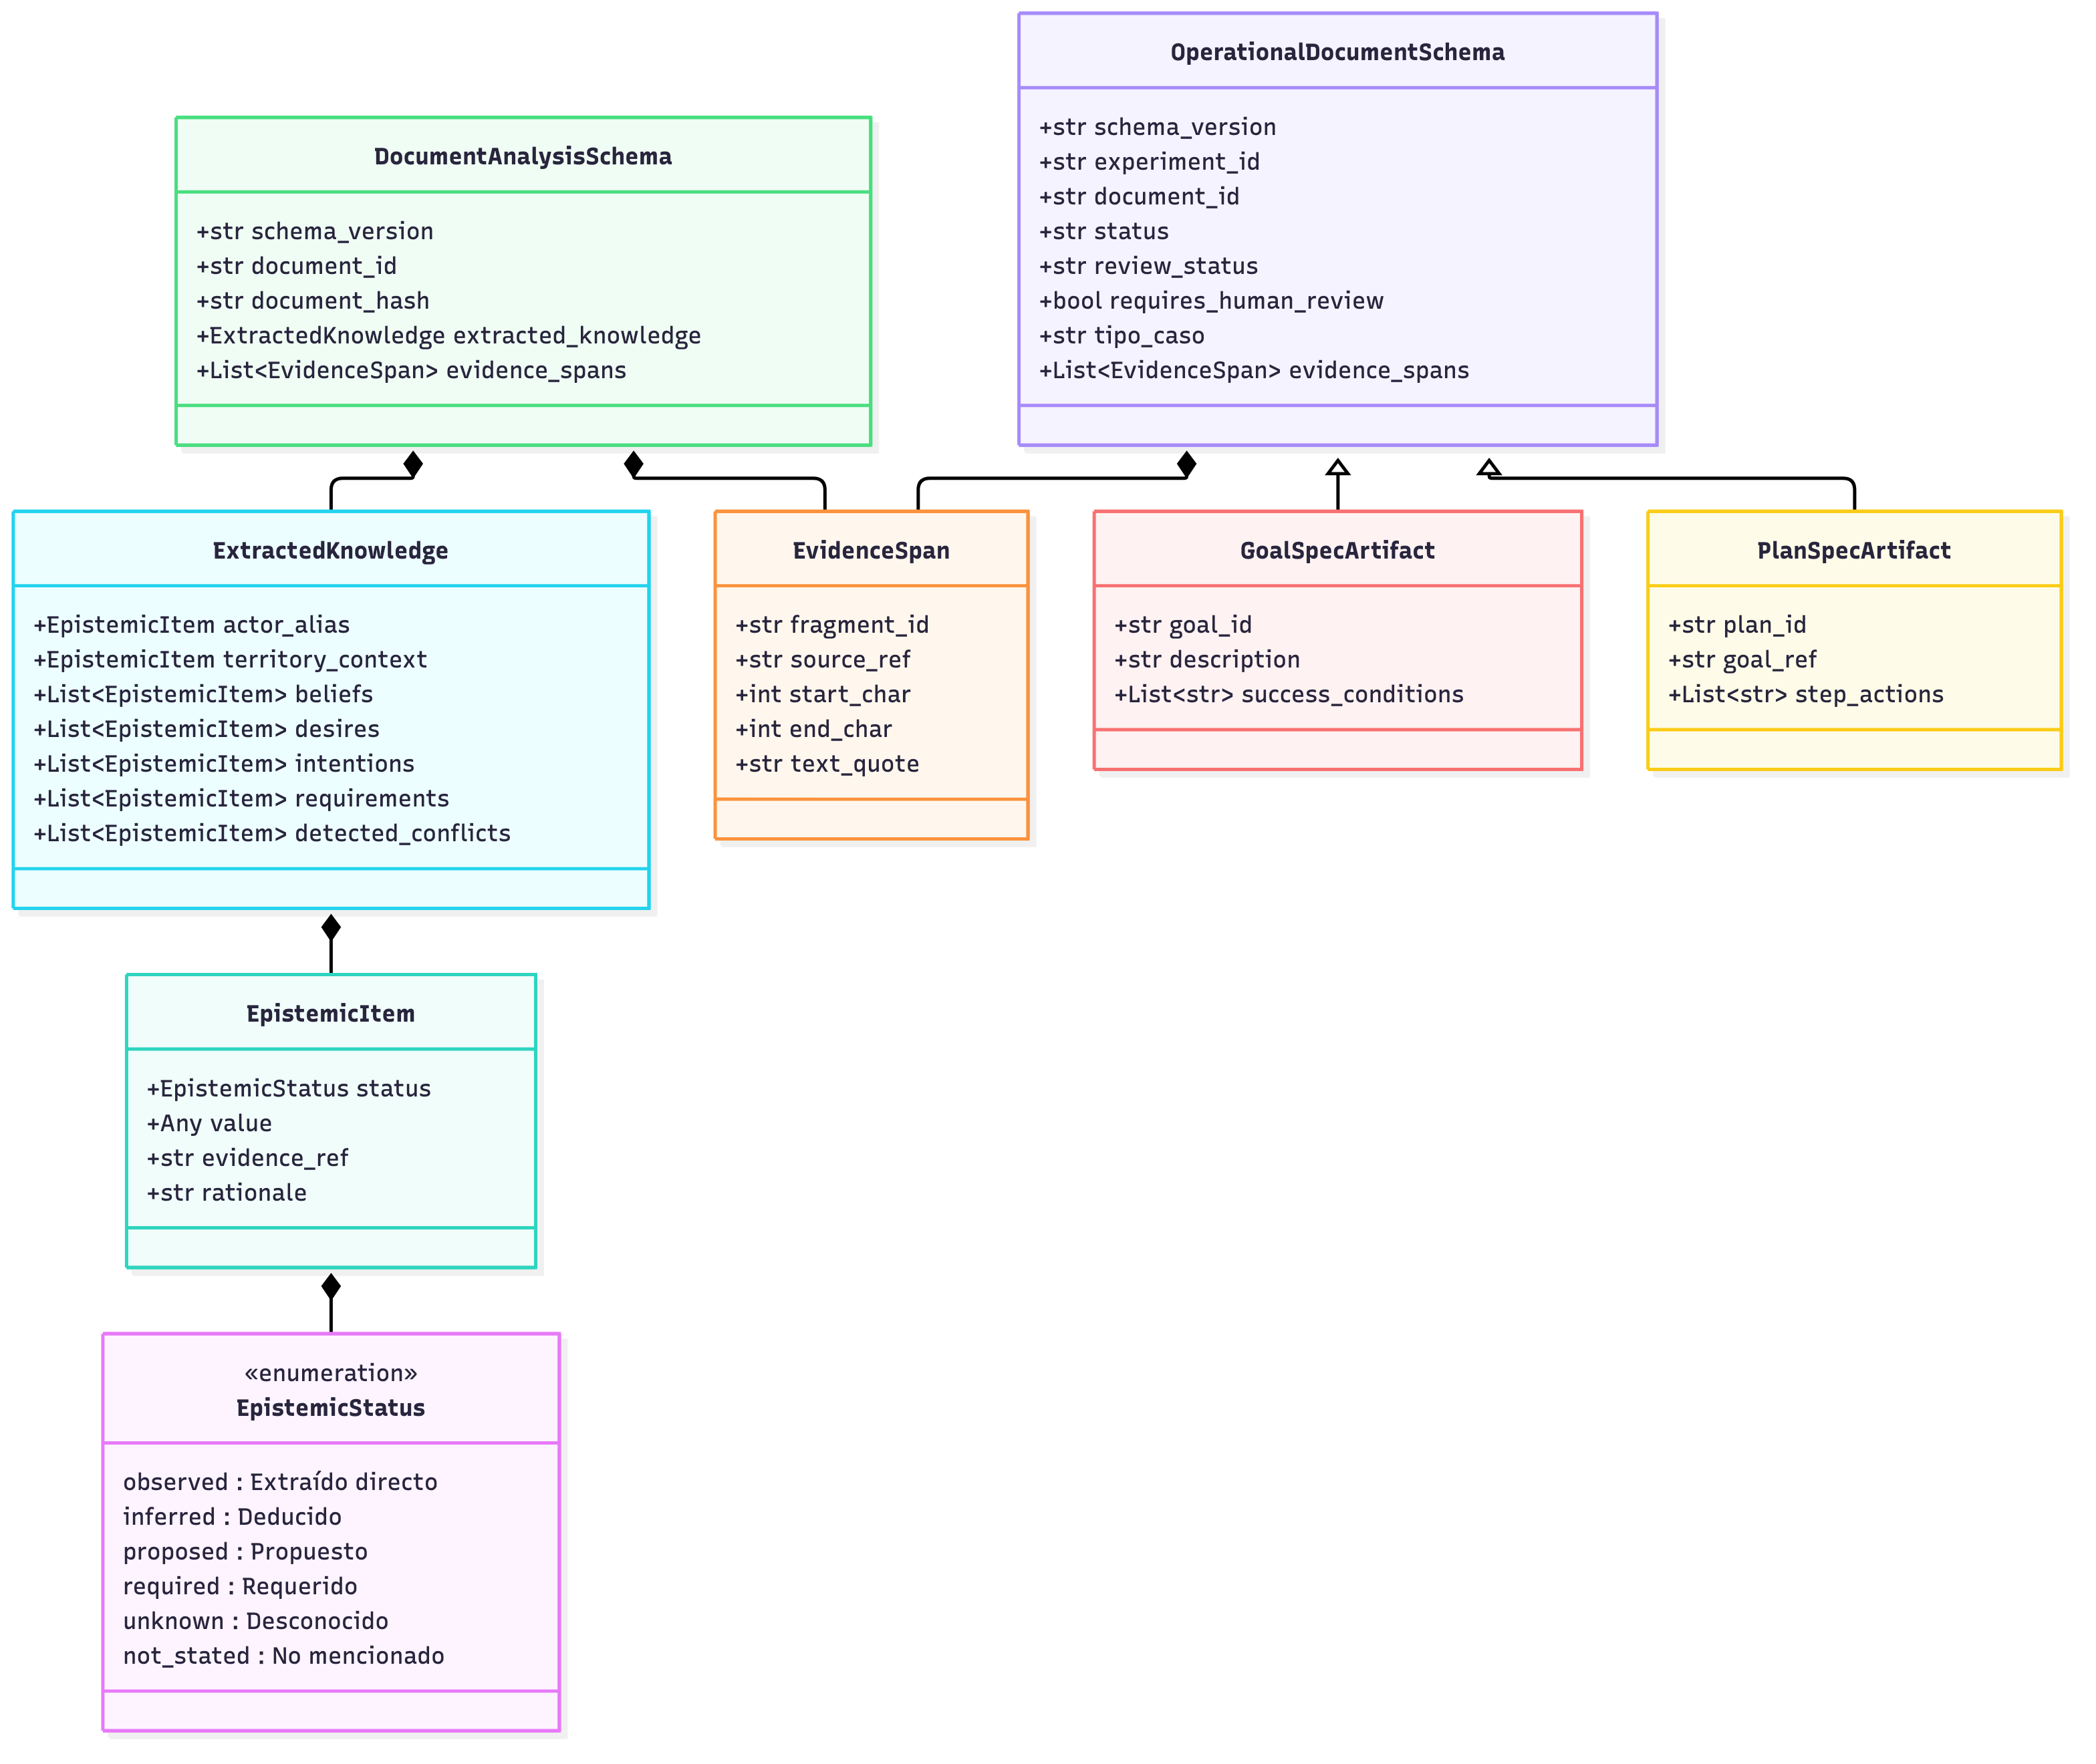
\includegraphics[width=0.92\textwidth,height=0.45\textheight,keepaspectratio]{figures/es/d08_data_model_contracts.png}
    \caption{Figura D8. Modelo de Datos y Contratos Formales. Estructura de esquemas validados para Caso Puro (\texttt{CasoPuro}) y Caso Conflictivo (\texttt{CasoConflictivo}).}
    \label{fig:d08_data_model}
\end{figure}

\subsection{Persistencia Atómica y Resiliencia de Disco}
El servicio \texttt{ManualIntentService} (\texttt{apps/api/src/application/manual\_intent\_service.py}) asegura escrituras atómicas en disco cumpliendo las garantías POSIX:
\begin{enumerate}
    \item Escribe un archivo temporal (\texttt{temp\_path}) anexando un sufijo UUID aleatorio (\texttt{.tmp.<hex>}).
    \item Fuerza el vaciado de buffers y sincronización física en disco mediante \texttt{f.flush()} y \texttt{os.fsync(f.fileno())}.
    \item Renombra atómicamente mediante reemplazo POSIX con \texttt{os.replace(temp\_path, target\_path)}.
    \item Cláusula \texttt{finally}: si ocurre cualquier anomalía previa al renombrado, el archivo temporal se destruye inmediatamente, garantizando que el archivo anterior no sufra corrupción.
\end{enumerate}

\subsection{Borrado Lógico y Retención de 30 Días}
Al invocar \texttt{DELETE /v2/intents/\{id\}}, el archivo no es purgado físicamente. Se lee su contenido, se incrementa su metadata inyectando el bloque \texttt{trash\_metadata}:
\begin{lstlisting}[language=Python]
trash_meta = {
    "deleted_at": datetime.now(timezone.utc).isoformat(),
    "deleted_by": deleted_by,
    "retention_days": 30,
    "expires_at": (datetime.now(timezone.utc) + timedelta(days=30)).isoformat(),
    "is_expired": False
}
\end{lstlisting}
El archivo es transferido atómicamente a \texttt{outputs/intents/.trash/\{id\}.json}. Dentro de este periodo, puede ser restaurado (\texttt{POST /v2/intents/\{id\}/restore}). Si se intenta restaurar un elemento cuya fecha actual supera \texttt{expires\_at}, el endpoint retorna \textbf{HTTP 410 Gone}.

\subsection{Purga Programada de Vencidos}
La depuración física definitiva se desencadena bajo demanda (\texttt{POST /v2/intents/trash/purge} o \texttt{make purge-trash}) y durante el arranque del servidor FastAPI (\textit{lifespan hook} en \texttt{src/api/main.py}). Solo se eliminan archivos cuyo cálculo \texttt{now >= expires\_at} sea verdadero.

% ==============================================================================
% 11. RESULTADOS DE IMPLEMENTACIÓN
% ==============================================================================
\section{Resultados de Implementación}

\subsection{Endpoints REST Habilitados}
La API expone bajo el enrutador \texttt{/v2/intents} ocho operaciones completamente probadas:
\begin{itemize}[itemsep=1pt]
    \item \texttt{POST /v2/intents}: Creación estricta (HTTP 201). Rechaza duplicados con HTTP 409.
    \item \texttt{GET /v2/intents}: Listado consolidado de intenciones activas (HTTP 200).
    \item \texttt{GET /v2/intents/\{id\}}: Consulta por identificador único (HTTP 200 / 404).
    \item \texttt{PUT /v2/intents/\{id\}}: Edición versionada con cálculo de nuevo SHA-256 (HTTP 200 / 404 / 422).
    \item \texttt{DELETE /v2/intents/\{id\}}: Borrado lógico hacia \texttt{.trash/} (HTTP 200 / 404).
    \item \texttt{GET /v2/intents/trash}: Listado de intenciones en papelera de reciclaje (HTTP 200).
    \item \texttt{POST /v2/intents/\{id\}/restore}: Restauración al almacén activo (HTTP 200 / 409 / 410).
    \item \texttt{POST /v2/intents/trash/purge}: Purga de elementos que superaron los 30 días (HTTP 200).
\end{itemize}

\subsection{Interfaz Web en React y Experiencia de Usuario}
Se desarrolló el componente \texttt{ManualIntentsView.tsx} integrado en la interfaz de Vite:
\begin{itemize}[itemsep=2pt]
    \item \textbf{Panel KPI de Cabecera:} Indicadores en vivo de intenciones activas, desglose Puro/Conflicto, conteo de papelera y estado de conectividad con la API.
    \item \textbf{Plantillas a 1 Clic:} Carga de estructuras agronómicas válidas para labranza mínima (Puro) y dilema de cuotas de riego (Conflicto).
    \item \textbf{Papelera de 30 Días:} Barra de progreso visual con conteo regresivo de días restantes antes de la purga física y botón de restauración inmediata.
    \item \textbf{Compilación y Calidad:} Compilación de producción con Vite en 213~ms y análisis estático con \texttt{oxlint} en 26~ms con 0 errores y 0 advertencias.
\end{itemize}

La interfaz web fue ejecutada y revisada manualmente en el navegador local. Se verificaron los flujos de creación, consulta, edición, borrado lógico, consulta de la papelera, restauración y purga de intenciones. También se comprobó la visualización de los casos Caso Puro y Caso Conflictivo, incluyendo sus campos específicos y los mensajes de respuesta de la API. Los flujos observados coincidieron con el comportamiento esperado definido para el Bloque B5.

% ==============================================================================
% 12. RESULTADOS DE AUDITORÍA
% ==============================================================================
\section{Resultados de Auditoría}

La auditoría técnica formal se ejecutó de forma reproducible sobre un directorio temporal aislado (\texttt{tmp\_path}). A continuación se presenta la matriz de aceptación correspondiente a los criterios B5-01 a B5-24:

\begin{table}[H]
\centering
\small
\begin{tabularx}{\textwidth}{p{1.1cm}p{3.3cm}Xp{1.5cm}p{3.2cm}}
\toprule
\textbf{ID} & \textbf{Criterio} & \textbf{Evidencia Exigida} & \textbf{Estado} & \textbf{Observación} \\
\midrule
B5-01 & Crear Caso Puro & POST HTTP 201, persistencia en disco & CUMPLE & Versión 1, hash canónico \\
B5-02 & Crear Caso Conflictivo & POST HTTP 201, contrato validado & CUMPLE & Fuentes y opciones intactas \\
B5-03 & Validar datos inválidos & HTTP 422 ante campos extra o erróneos & CUMPLE & \texttt{extra="forbid"} activo \\
B5-04 & No sobrescritura & HTTP 409 ante ID duplicado & CUMPLE & Archivo previo protegido \\
B5-05 & Editar intención & PUT HTTP 200 con versión incrementada & CUMPLE & Versión pasa de 1 a 2 \\
B5-06 & Edición inválida & HTTP 422 ante esquema corrupto & CUMPLE & Archivo previo inalterado \\
B5-07 & Listar y consultar & GET HTTP 200 en endpoints de lectura & CUMPLE & Integridad de payloads \\
B5-08 & Borrado lógico & Traslado a \texttt{.trash/} con metadatos & CUMPLE & 100\% en papelera (4/4) \\
B5-09 & Retención de 30 días & Bloqueo de purga si $t < 30\text{d}$ & CUMPLE & Prueba temporal simulada \\
B5-10 & Purga de vencidos & Eliminación física si $t \ge 30\text{d}$ & CUMPLE & Purgado definitivo verificado \\
B5-11 & Restauración & Reincorporación a directorio activo & CUMPLE & Retiro de \texttt{.trash/} \\
B5-12 & Conflicto restauración & HTTP 409 si el ID fue reutilizado & CUMPLE & Detección de colisión \\
B5-13 & Bloqueo Path Traversal & 100\% rechazo en casos negativos (5/5) & CUMPLE & Regex estricta \\
B5-14 & Bloqueo de Symlinks & HTTP 403 ante enlaces simbólicos & CUMPLE & \texttt{Path.is\_symlink()} \\
B5-15 & Escritura confinada & Confinamiento en \texttt{outputs/intents/} & CUMPLE & Restricción de prefijo \\
B5-16 & Atomicidad en fallos & Fallo en \texttt{os.replace} conserva estado & CUMPLE & Archivo base intacto \\
B5-17 & Temporales huérfanos & 0 temporales tras fallo inducido & CUMPLE & Cláusula \texttt{finally} \\
B5-18 & Trazabilidad auditoría & Eventos en \texttt{audit.log} append-only & CUMPLE & 14/14 eventos registrados \\
B5-19 & Integridad de Hash & SHA-256 canónico determinista & CUMPLE & Normalización de claves \\
B5-20 & Núcleo protegido & 0 escrituras en simulador externo & CUMPLE & 514 archivos, hash idéntico \\
B5-21 & Códigos de API & Respuestas 200, 201, 403, 404, 409, 410, 422 & CUMPLE & TestClient automatizado \\
B5-22 & Interfaz de Usuario & Código, contratos TypeScript, build, lint, pruebas HTTP y validación manual en navegador & CUMPLE & Flujos conformes al diseño de B5 \\
B5-23 & No regresión & Suite global de pruebas sin fallos & CUMPLE & 79/79 pruebas aprobadas \\
B5-24 & Gobierno de Git & Working tree auditado sin commits no autorizados & CUMPLE & Reglas 9 y 10 observadas \\
\bottomrule
\end{tabularx}
\caption{Matriz de Aceptación del Bloque B5. Cumplimiento de criterios funcionales y de seguridad.}
\label{tab:matriz_b5}
\end{table}

% ==============================================================================
% 13. SEGURIDAD Y TRAZABILIDAD
% ==============================================================================
\section{Seguridad y Trazabilidad}

\subsection{Validación Negativa de Entradas}
Se obtuvo un \textbf{rechazo del 100\% sobre los 16 casos negativos evaluados} (16/16). La Tabla~\ref{tab:casos_negativos} desglosa cada vector de prueba, el código HTTP resultante y el mecanismo de mitigación activado.

\begin{table}[H]
\centering
\small
\begin{tabularx}{\textwidth}{llccX}
\toprule
\textbf{\#} & \textbf{Caso Negativo Evaluado} & \textbf{HTTP} & \textbf{Estado} & \textbf{Mecanismo de Mitigación} \\
\midrule
1 & Identificador vacío (\texttt{""}) & 422 & PASS & Validación de longitud mínima Pydantic \\
2 & Identificador con espacios intermedios & 422 & PASS & Rechazo por patrón regex \\
3 & Path traversal con \texttt{../} & 422 & PASS & Detección sintáctica de secuencia de escape \\
4 & Separador de ruta POSIX (\texttt{/}) & 422 & PASS & Prohibición de caracteres de jerarquía \\
5 & Separador de ruta Windows (\texttt{\textbackslash}) & 422 & PASS & Prohibición de barras invertidas \\
6 & Ruta absoluta (\texttt{/etc/intento}) & 422 & PASS & Prohibición de diagonales iniciales \\
7 & Enlace simbólico forzado & 403 & PASS & Detección explícita con \texttt{is\_symlink()} \\
8 & Longitud mayor a 64 caracteres & 422 & PASS & Límite estricto \texttt{max\_length=64} \\
9 & Payload con campo extra & 422 & PASS & Configuración \texttt{extra="forbid"} \\
10 & Payload sin campo obligatorio & 422 & PASS & Ausencia de bloque discriminado \texttt{intent} \\
11 & Tipo de caso inválido (\texttt{magico}) & 422 & PASS & Discriminador de unión \texttt{puro}/\texttt{conflicto} \\
12 & Edición de ID inexistente & 404 & PASS & Captura de \texttt{IntentNotFoundError} \\
13 & Borrado de ID inexistente & 404 & PASS & Verificación previa de existencia \\
14 & Restauración inexistente & 404 & PASS & Ausencia de registro en \texttt{.trash/} \\
15 & Restauración vencida ($>30\text{d}$) & 410 & PASS & Evaluación de caducidad temporal \\
16 & Duplicación de ID en creación & 409 & PASS & Control de colisión con \texttt{FileExistsError} \\
\bottomrule
\end{tabularx}
\caption{Resultados de la Validación Negativa de Entradas en el Bloque B5.}
\label{tab:casos_negativos}
\end{table}

\subsection{Verificación Criptográfica del Núcleo Protegido}
Para confirmar que el CRUD de intenciones no altera el simulador de producción, se auditó directamente el directorio externo:
\begin{center}
\texttt{/Volumes/ADATA SD620/Programacion 7.0/universidad/proyecto de grado/EthosTerra}
\end{center}
Dicha ruta corresponde al repositorio independiente del simulador que aloja el núcleo BESA en Python, scripts de simulación y documentación de diseño. La verificación se ejecutó mediante los siguientes comandos reproducibles:
\begin{lstlisting}[language=bash]
# Inventario de archivos regulares
find "/Volumes/ADATA SD620/Programacion 7.0/universidad/proyecto de grado/EthosTerra" -type f | wc -l
# Calculo de hash combinado determinista
python3 -c '
import hashlib, sys
from pathlib import Path
target = Path("/Volumes/ADATA SD620/Programacion 7.0/universidad/proyecto de grado/EthosTerra")
files = sorted([p for p in target.rglob("*") if p.is_file()])
h = hashlib.sha256()
for f in files:
    h.update(str(f.relative_to(target)).encode("utf-8"))
    h.update(f.read_bytes())
print(f"Total: {len(files)} files | Hash: {h.hexdigest()}")
'
\end{lstlisting}

\textbf{Resultado comparativo:}
\begin{itemize}[itemsep=1pt]
    \item Archivos antes de las pruebas: \textbf{514}
    \item Archivos después de las pruebas: \textbf{514}
    \item Hash SHA-256 antes: {\scriptsize\texttt{f182c62ebeb1bc85b49b3975366bf56ed062af775ed91ac63d0ef9ce65537a8a}}
    \item Hash SHA-256 después: {\scriptsize\texttt{f182c62ebeb1bc85b49b3975366bf56ed062af775ed91ac63d0ef9ce65537a8a}}
    \item Conclusión: \textbf{$\text{escrituras\_nucleo} = 0$}. El 100\% de los archivos permaneció inalterado.
\end{itemize}

% ==============================================================================
% 14. MÉTRICAS
% ==============================================================================
\section{Métricas}

\subsection{Métricas Cuantitativas del Bloque B5}
La Tabla~\ref{tab:metricas_b5} presenta los resultados cuantitativos obtenidos en la auditoría con denominadores explícitos.

\begin{table}[H]
\centering
\small
\begin{tabularx}{\textwidth}{p{3.8cm}Xccr}
\toprule
\textbf{Métrica de Evaluación} & \textbf{Expresión de Cálculo} & \textbf{Num. / Den.} & \textbf{Porcentaje} & \textbf{Meta} \\
\midrule
Tasa de creación válida & Creaciones exitosas / Intentos válidos & 2 / 2 & 100.0\% & 100\% \\
Tasa de rechazo negativo & Rechazos conformes / Casos negativos & 16 / 16 & 100.0\% & 100\% \\
Tasa de edición versionada & Ediciones exitosas / Intentos válidos & 2 / 2 & 100.0\% & 100\% \\
Tasa de borrado lógico & Borrados a papelera / Borrados normales & 4 / 4 & 100.0\% & 100\% \\
Tasa de retención 30 días & Retenciones respetadas / Casos $<30\text{d}$ & 2 / 2 & 100.0\% & 100\% \\
Tasa de purga física & Purgas de vencidos / Casos $\ge 30\text{d}$ & 2 / 2 & 100.0\% & 100\% \\
Tasa de restauración & Restauraciones exitosas / Intentos en ventana & 2 / 2 & 100.0\% & 100\% \\
Tasa de bloqueo de escape & Escapes neutralizados / Ataques de ruta & 5 / 5 & 100.0\% & 100\% \\
Tasa de bloqueo symlink & Enlaces bloqueados / Ataques symlink & 1 / 1 & 100.0\% & 100\% \\
Tasa de atomicidad & Fallos sin huérfanos / Fallos inducidos & 3 / 3 & 100.0\% & 100\% \\
Tasa de trazabilidad & Eventos auditados / Mutaciones ejecutadas & 14 / 14 & 100.0\% & 100\% \\
Escrituras al núcleo & Creados + Modificados + Eliminados & 0 / 514 & 0 & 0 \\
\bottomrule
\end{tabularx}
\caption{Métricas Cuantitativas de Seguridad, Persistencia y Operación de B5.}
\label{tab:metricas_b5}
\end{table}

\subsection{Clasificación de Evidencia por Origen}
La Tabla~\ref{tab:origen_evidencia} delimita qué evidencia fue generada durante la Semana 8 y qué componentes corresponden a líneas base preexistentes.

\begin{table}[H]
\centering
\small
\begin{tabularx}{\textwidth}{lp{5.0cm}p{4.2cm}l}
\toprule
\textbf{Categoría} & \textbf{Componentes Evaluados} & \textbf{Método de Verificación} & \textbf{Estado} \\
\midrule
\textbf{Semana 8 (B5)} & CRUD manual, papelera, retención 30d, purga, atomicidad, hash, UI & 26 pruebas B5, runner aislado, inventario núcleo & Validados \\
\textbf{Heredados (S5--S7)} & Approval Gate, clasificador híbrido, hooks de dominio, sandbox exp\_001 & 53 pruebas baseline, reporte Semana 5 & Inmutables \\
\textbf{Inspección estática} & Contratos Pydantic V2, regex de identificadores, linter de UI & \texttt{extra="forbid"}, \texttt{oxlint} (26ms), \texttt{tsc -b} & Cumple \\
\textbf{Automatizadas} & Endpoints REST, códigos HTTP, ciclo de vida & \texttt{TestClient}, \texttt{pytest} (79 pruebas en 0.35s) & Cumple \\
\textbf{Revisión en navegador} & Experiencia de usuario y flujos B5 & Inspección en \texttt{localhost:5173} & Cumple \\
\bottomrule
\end{tabularx}
\caption{Clasificación y Separación de Evidencia Experimental por Origen.}
\label{tab:origen_evidencia}
\end{table}

\subsection{Visualización Gráfica de Pruebas y Estados}
A continuación se ilustra cuantitativamente el resultado de las pruebas automatizadas ejecutadas durante la auditoría.

\begin{figure}[H]
\centering
\begin{tikzpicture}
\begin{axis}[
    ybar,
    bar width=14pt,
    width=0.88\textwidth,
    height=5.0cm,
    enlargelimits=0.15,
    ylabel={Cantidad de Pruebas},
    symbolic x coords={Suite Global, Suite B5, Negativos, Atomicidad},
    xtick=data,
    nodes near coords,
    nodes near coords align={vertical},
    legend style={at={(0.5,-0.25)}, anchor=north, legend columns=-1},
    ymajorgrids=true,
    grid style=dashed
]
\addplot[fill=darkgreen!80!black] coordinates {(Suite Global, 79) (Suite B5, 26) (Negativos, 16) (Atomicidad, 3)};
\addplot[fill=warnred!80!black] coordinates {(Suite Global, 0) (Suite B5, 0) (Negativos, 0) (Atomicidad, 0)};
\legend{Aprobadas (Passed), Fallidas (Failed)}
\end{axis}
\end{tikzpicture}
\caption{Distribución de Pruebas Automatizadas Aprobadas frente a Fallidas.}
\label{fig:chart_tests}
\end{figure}

El autómata de estados finitos que gobierna el ciclo de vida de las intenciones manuales se representa en la Figura~\ref{fig:lifecycle_diagram}.

\begin{figure}[H]
\centering
\begin{tikzpicture}[
    node distance=2.2cm,
    state/.style={rectangle, rounded corners, draw=navyblue, fill=blue!5, thick, minimum width=2.8cm, minimum height=1.0cm, align=center},
    edge/.style={->, >=Stealth, thick, draw=navyblue},
    warnedge/.style={->, >=Stealth, thick, draw=warnred, dashed}
]
\node[state] (nuevo) {Entrada\\Declarativa};
\node[state, right=of nuevo] (activo) {Almacén Activo\\\texttt{outputs/intents/}};
\node[state, right=of activo] (papelera) {Papelera Temporal\\\texttt{.trash/} ($t < 30\text{d}$)};
\node[state, below=of papelera, draw=warnred, fill=red!5] (purgado) {Purga Física\\Definitiva};

\draw[edge] (nuevo) -- node[above]{\footnotesize POST /v2/intents} (activo);
\draw[edge] (activo) to[bend left=20] node[above]{\footnotesize DELETE} (papelera);
\draw[edge] (papelera) to[bend left=20] node[below]{\footnotesize POST /restore} (activo);
\draw[warnedge] (papelera) -- node[right]{\footnotesize $t \ge 30\text{d}$ (POST /purge)} (purgado);
\draw[edge] (activo) to[loop above] node[above]{\footnotesize PUT (Versionado)} (activo);
\end{tikzpicture}
\caption{Ciclo de Vida de Persistencia: Almacén Activo, Papelera Temporal y Purga Definitiva.}
\label{fig:lifecycle_diagram}
\end{figure}

% ==============================================================================
% 15. DISCUSIÓN
% ==============================================================================
\section{Discusión}

El diseño implementado en B5 valida la hipótesis de que es posible alcanzar robustez industrial y seguridad de grado forense sin incorporar complejidad accidental. El uso de archivos JSON locales combinados con primitivas atómicas del sistema operativo POSIX (\texttt{os.replace}) eliminó la necesidad de introducir un motor SQL o un almacén de claves (Redis), reduciendo a cero las dependencias de red externa y manteniendo la ejecución 100\% offline.

Una observación crítica derivada de la auditoría radica en el rigor de los contratos Pydantic V2: al haber estipulado \texttt{extra="forbid"}, cualquier desviación en la nomenclatura de la petición (por ejemplo, enviar \texttt{"created\_by"} en lugar de \texttt{"author"}) resulta en un bloqueo determinista con HTTP 422. De igual forma, en el Caso Conflictivo, restringir las fuentes en colisión a literales de dominio (\texttt{"context\_field"} y \texttt{"document"}) previene que descripciones libres degraden la semántica de la compuerta eBDI.

% ==============================================================================
% 16. LIMITACIONES
% ==============================================================================
\section{Limitaciones}

Se identifican las siguientes consideraciones y límites de alcance correspondientes a la etapa actual:
\begin{enumerate}[itemsep=2pt]
    \item \textbf{Integración con el simulador diferida a B7:} El módulo B5 gestiona intenciones en almacenamiento local; la ingestión y acoplamiento con el ciclo de deliberación del simulador WellProdSim / EthosTerra se ejecutará en las Semanas 10 a 12.
    \item \textbf{Pruebas integrales de simulación programadas para B9:} Las pruebas end-to-end con agentes eBDI activos y verificación de mutación de creencias corresponden al Bloque B9 (Semanas 12 y 13).
    \item \textbf{Purga ejecutada al inicio de la API o bajo demanda:} Para evitar la sobrecarga de demonios en segundo plano, la purga física de intenciones vencidas se activa en el arranque del servidor FastAPI o mediante invocación del endpoint correspondiente.
    \item \textbf{Verificación del simulador dependiente del volumen local:} La verificación de no escritura en el núcleo de \texttt{EthosTerra} se basa en la disponibilidad del volumen de desarrollo; en entornos donde no esté presente, la protección se garantiza mediante el confinamiento estricto de rutas en el código.
    \item \textbf{Validación con expertos programada para B10:} La evaluación semántica con un panel de agrónomos y extensionistas rurales está reservada formalmente para el Bloque B10 (Semanas 13 y 14).
\end{enumerate}

% ==============================================================================
% 17. ESTADO FRENTE AL CRONOGRAMA
% ==============================================================================
\section{Estado frente al Cronograma}

La Hoja de Ruta consolidada de los trece bloques de trabajo se detalla en la Figura~\ref{fig:d11_roadmap}. El Bloque B5 concluye dentro de la ventana temporal planificada (Semanas 8 y 9).

\begin{figure}[H]
    \centering
    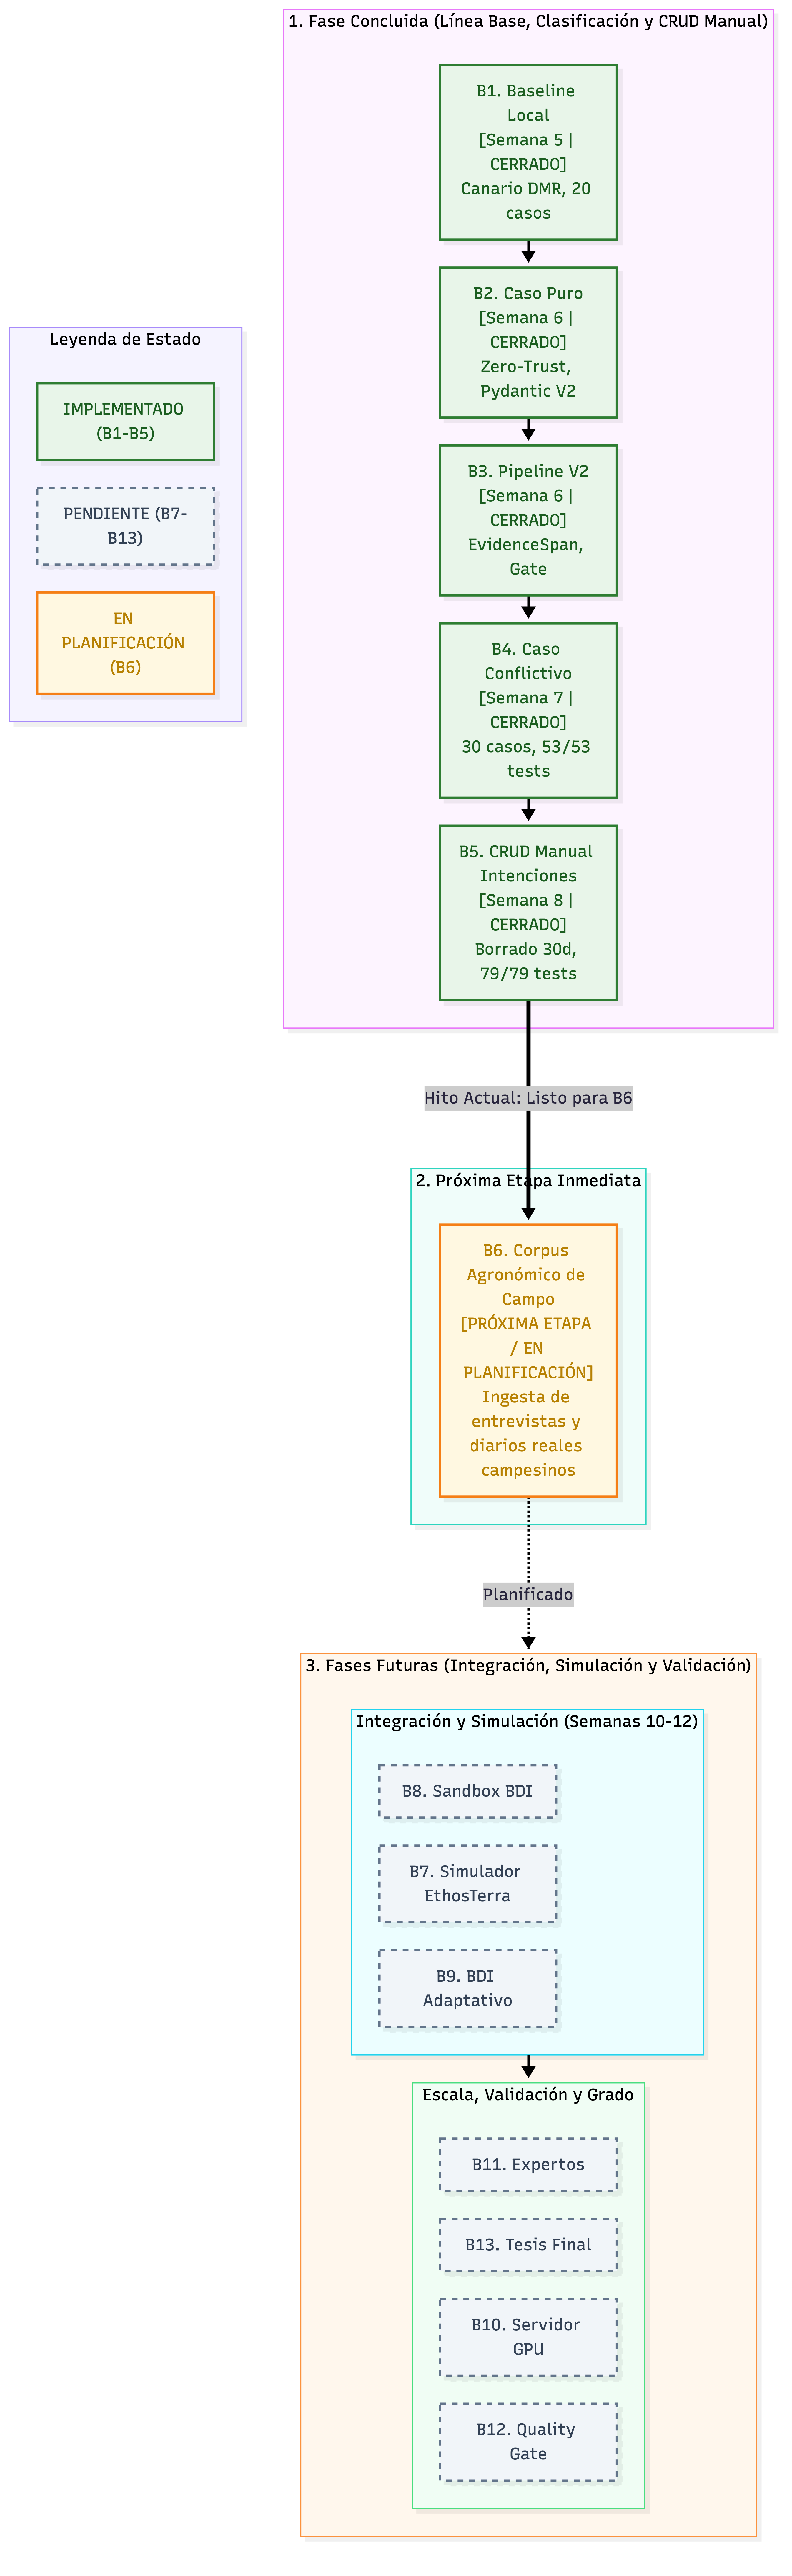
\includegraphics[width=0.92\textwidth,height=0.45\textheight,keepaspectratio]{figures/es/d11_status_roadmap.png}
    \caption{Figura D11. Mapa de Estado y Hoja de Ruta de Desarrollo (Bloques B1 a B13), reflejando la culminación del Bloque B5 y el inicio del Bloque B6.}
    \label{fig:d11_roadmap}
\end{figure}

El estado formal frente al cronograma semestral de la Fase 2 se presenta en la Tabla~\ref{tab:cronograma}.

\begin{table}[H]
\centering
\small
\begin{tabularx}{\textwidth}{p{1.8cm}p{4.5cm}ccX}
\toprule
\textbf{Bloque} & \textbf{Descripción Técnica} & \textbf{Semanas} & \textbf{Estado Formal} & \textbf{Comentarios} \\
\midrule
\textbf{B1--B3} & Clasificador Caso Puro & 1--5 & Cerrado & 20 casos evaluados con Gemma 4 \\
\textbf{B4} & Clasificador Caso Conflictivo & 6--7 & Cerrado & Matriz de colisión e informe S7 \\
\textbf{B5} & CRUD Manual de Intenciones & 8--9 & \textbf{Completado} & Auditoría y revisión manual aprobadas \\
\textbf{B6} & Pruebas con Corpus Agronómico & 9--10 & Pendiente & Ingesta de diarios de campo \\
\textbf{B7} & Integración con Simulador & 10--12 & Pendiente & Conexión con Python BESA \\
\textbf{B8} & Sistema Multiagente eBDI & 4--11 & En paralelo & Modelado de metas y planes \\
\textbf{B9} & Pruebas End-to-End & 12--13 & Pendiente & Simulación completa con rollback \\
\textbf{B10} & Validación Semántica Interna & 13--14 & Pendiente & Preparación para panel de expertos \\
\textbf{B11--B13} & Consolidación y Sustentación & 14--16 & Pendiente & Tesis de maestría \\
\bottomrule
\end{tabularx}
\caption{Estado Actual del Cronograma Semestral de Investigación (Fase 2).}
\label{tab:cronograma}
\end{table}

% ==============================================================================
% 18. TRABAJO PENDIENTE
% ==============================================================================
\section{Trabajo Pendiente}

Para dar paso formal al Bloque B6, se establecen las siguientes acciones prioritarias:
\begin{enumerate}[itemsep=2pt]
    \item Realizar la inspección pre-commit obligatoria y solicitar autorización para congelar el incremento de Semana 8 en Git.
    \item Recolectar y normalizar el corpus de textos y diarios agronómicos de pequeños productores campesinos para la suite de pruebas del Bloque B6.
    \item Diseñar las pruebas de carga y estrés para el almacenamiento de intenciones en lotes superiores a 100 archivos concurrentes.
    \item Estructurar las interfaces de acoplamiento preliminares para la integración del Bloque B7 frente a Python BESA.
\end{enumerate}

% ==============================================================================
% 19. CONCLUSIONES
% ==============================================================================
\section{Conclusiones}

La Semana 8 permitió completar el Bloque B5 del proyecto. El CRUD manual de intenciones quedó funcional para los casos Puro y Conflictivo, con persistencia JSON, control de versiones, borrado lógico, retención, restauración, purga, validación de entradas, escritura atómica, auditoría y protección de rutas. Las pruebas automatizadas y la revisión manual de la interfaz confirmaron el comportamiento esperado. El bloque queda completado y el trabajo siguiente corresponde a las actividades de integración y pruebas definidas para las semanas posteriores.

El estado técnico oficial del incremento es \textbf{B5 COMPLETADO}.

% ==============================================================================
% 20. REFERENCIAS
% ==============================================================================
\section{Referencias}

\begin{enumerate}[itemsep=2pt]
    \item Bratman, M. (1987). \textit{Intentions, Plans, and Practical Reason}. Harvard University Press.
    \item Rao, A. S., \& Georgeff, M. P. (1995). BDI agents: From theory to practice. \textit{Proceedings of the First International Conference on Multi-Agent Systems (ICMAS-95)}, 312--319.
    \item WellProdSim Development Team. (2025). \textit{WellProdSim: Agronomic Multi-Agent Simulation Environment}. Especificaciones de diseño interno.
    \item Martínez Velandia, J. A. (2026). \textit{Informe de Avance Experimental -- Semana 7 (Bloque B4): Implementación del clasificador de Caso Conflictivo}. Universidad Tecnológica de Bolívar.
    \item Pydantic Documentation. (2026). \textit{Data validation and settings management using Python type annotations}. Versión 2.13.
    \item FastAPI Framework. (2026). \textit{High performance, easy to learn, fast to code, ready for production}.
\end{enumerate}

% ==============================================================================
% 21. ANEXOS TÉCNICOS
% ==============================================================================
\section{Anexos Técnicos}

\subsection{Anexo A: Comandos de Operación y Makefile}
Para reproducir la totalidad de pruebas y levantar los servicios localmente, el repositorio provee las siguientes metas estandarizadas en el \texttt{Makefile}:
\begin{lstlisting}[language=bash]
# Ejecutar suite de pruebas de intenciones B5 (26 pruebas)
make test-b5

# Ejecutar suite unitaria completa sin regresiones (79 pruebas)
make test-unit

# Iniciar backend (puerto 8000) y frontend (puerto 5173) concurrentemente
make dev

# Purga bajo demanda de intenciones expiradas (>30 dias)
make purge-trash
\end{lstlisting}

\subsection{Anexo B: Estructura Canónica de un Caso Conflictivo Persistido}
A continuación se ilustra un archivo real persistido en \texttt{outputs/intents/agro\_conflicto\_riego\_cuota.json}:
\begin{lstlisting}[basicstyle=\ttfamily\scriptsize]
{
  "id": "agro_conflicto_riego_cuota",
  "intent": {
    "tipo": "conflicto",
    "conflicto_detectado": "Incompatibilidad entre limite comunal de consumo hidrico y estres severo.",
    "opciones_resolucion": [
      "Respetar turno comunal y posponer riego a horas nocturnas",
      "Riego de socorro localizado por goteo",
      "Solicitar ampliacion temporal de cuota ante junta de regantes"
    ],
    "requiere_humano": true,
    "descripcion_contradiccion": "Dilema entre estres hidrico y veda comunal.",
    "fuentes_en_colision": [
      {
        "source_type": "context_field",
        "source_id": "soil_moisture_level",
        "intencion": "regar_inmediato",
        "efecto": "mitigar_estres_hidrico",
        "evidence_ref": "telemetria_sensor_p2"
      },
      {
        "source_type": "document",
        "source_id": "estatuto_riego_comunal",
        "intencion": "racionar_consumo",
        "efecto": "evitar_sancion_y_desabastecimiento",
        "evidence_ref": "estatuto_2026_cap3"
      }
    ],
    "confidence": 1.0,
    "razonamiento": "Contradiccion insalvable entre telemetria de campo y acuerdo comunitario."
  },
  "metadata": {
    "created_at": "2026-10-02T10:46:14.355624Z",
    "created_by": "revisor_normativo",
    "updated_at": "2026-10-02T10:46:14.355624Z",
    "updated_by": "revisor_normativo",
    "canonical_hash": "7a4814d0b2f557c8e3c6dc69c424441d1a6274f231a5bc94f9f9b61ffc6f70e6",
    "version": 1
  }
}
\end{lstlisting}

\subsection{Anexo C: Instrucciones de Compilación del Documento}
Este informe puede ser compilado de forma independiente mediante cualquiera de las siguientes opciones:
\begin{lstlisting}[language=bash]
# Opcion 1: Con latexmk (recomendada)
latexmk -pdf -interaction=nonstopmode informe_semana_8_es.tex

# Opcion 2: Con pdflatex directo
pdflatex -interaction=nonstopmode informe_semana_8_es.tex
pdflatex -interaction=nonstopmode informe_semana_8_es.tex
\end{lstlisting}

\end{document}
